\documentclass[a4paper]{article}
\usepackage{flare}

\usepackage{ntheorem}
\theorembodyfont{\upshape}
\newtheorem{example}{Example}

\usepackage[x11names]{xcolor}
\usepackage{listings}
\lstset{%
  basicstyle=\ttfamily,
  flexiblecolumns,
  backgroundcolor=\color{Khaki1},
  xleftmargin=6pt,
  xrightmargin=6pt,
  gobble=3,
}


\begin{document}

Flare is a \LaTeX\ package and an extension to \texttt{\string\includegraphics}.
It is desinged for \texttt{lualatex} and does not support any other
\TeX-engine.

Note that Flare stores certain annotation data in an auxiliary \texttt{.flr}
file which serves the same purpose as \LaTeX's \texttt{.aux} file. To get
annotation data right it is necessary to run \texttt{lualatex} at least twice.

Here are some examples how to use Flare:

\begin{example}
  Simply copying all annotations. This is the default behavior, no
  Flare specific options needed.
  \begin{lstlisting}
    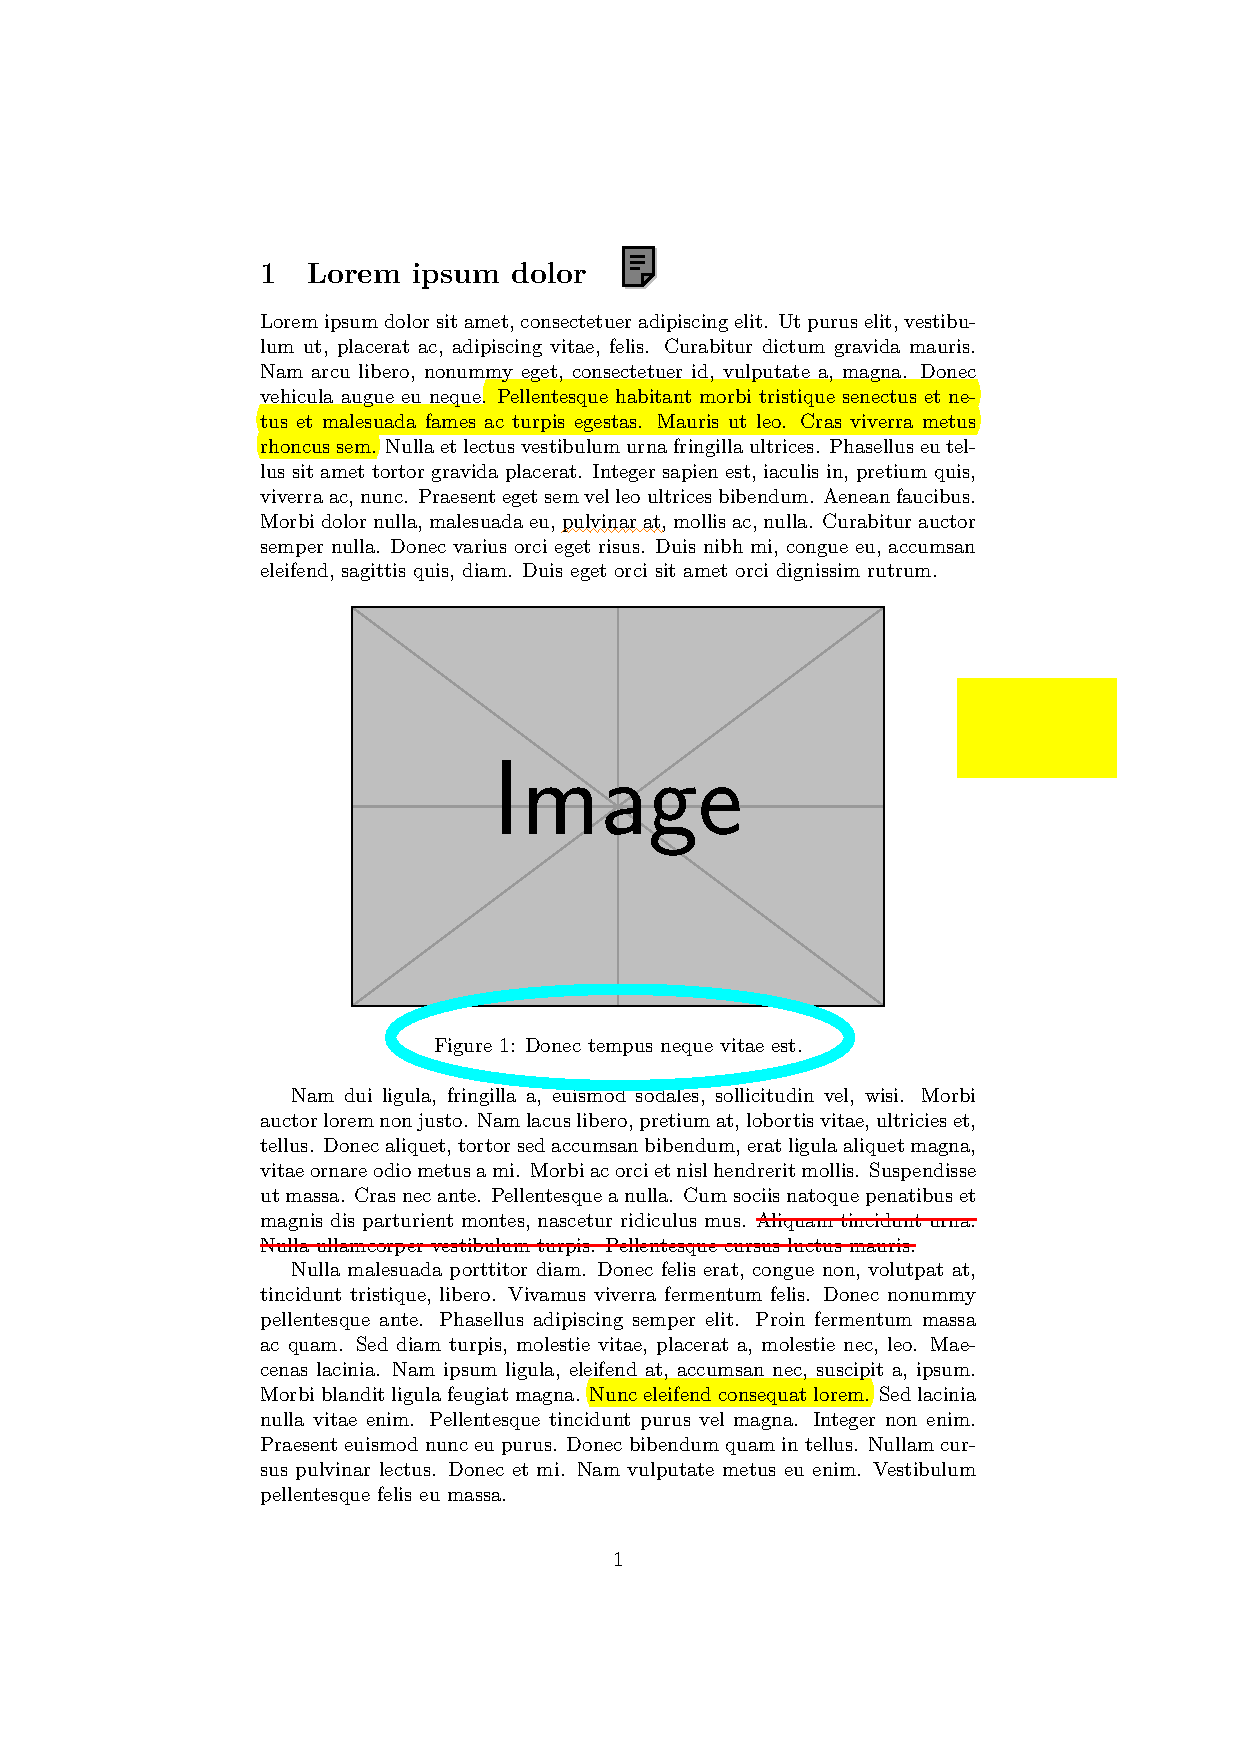
\includegraphics[scale=.5]{dummy-1.pdf}
  \end{lstlisting}
  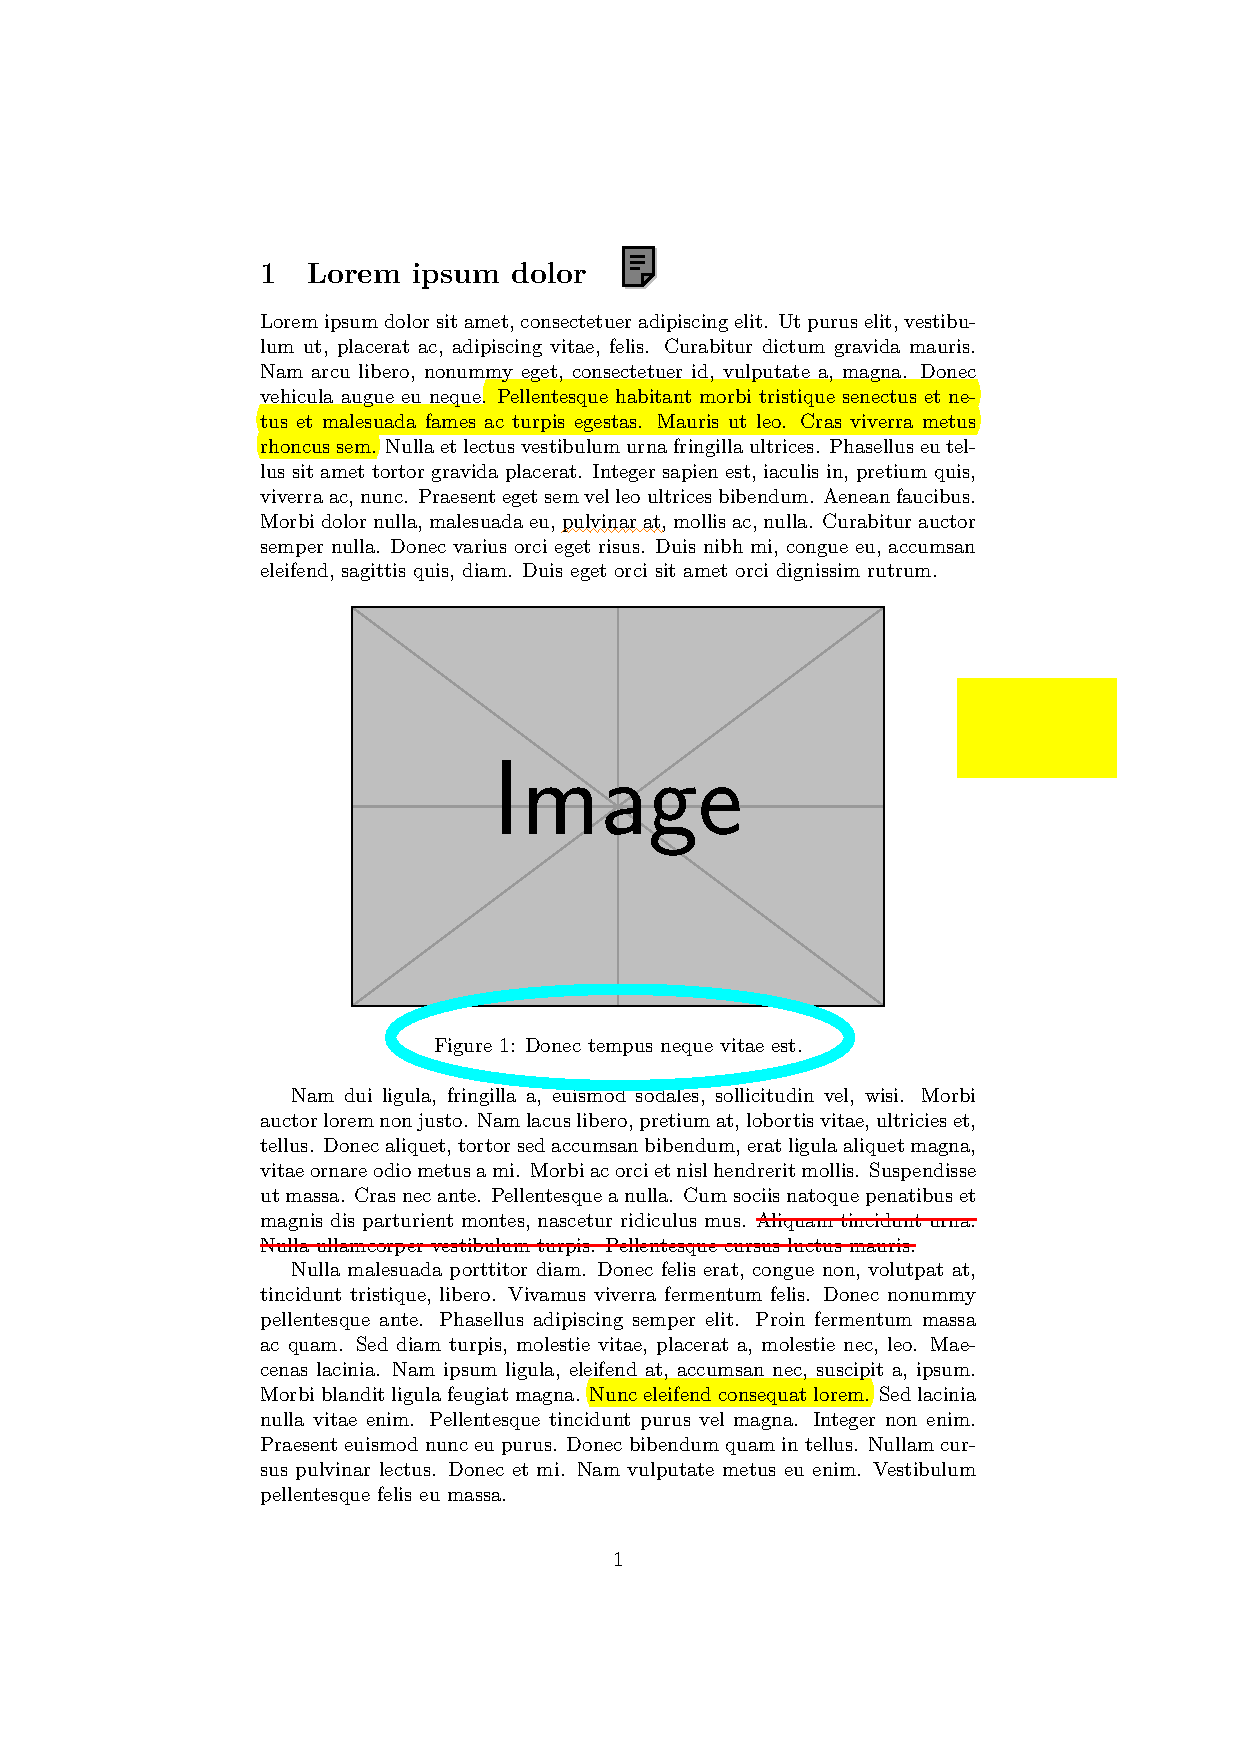
\includegraphics[scale=.5]{dummy-1.pdf}
\end{example}

\newpage
\begin{example}
  Replacing the color of all annotations. (Actually replacing the value
  of the \texttt{/C}-key in all annotations.)

  Syntax for replacing other keys: \texttt{flareReplace<PDF-Key> = \{...\}}
  
  \begin{lstlisting}
    \includegraphics[
       scale=0.5,
       flareReplaceC={[1 0 1]}
    ]{dummy-1.pdf}
  \end{lstlisting}
  \includegraphics[scale=0.5, flareReplaceC={[1 0 1]}]{dummy-1.pdf}
\end{example}

\newpage
\begin{example}
  Replacing the color of the 2nd and the 5th annotation.
  \begin{lstlisting}
    \includegraphics[
       scale=0.5,
       flareReplaceC!2={[0 1 0]},
       flareReplaceC!5={[1 0 1]}
    ]{dummy-1.pdf}
  \end{lstlisting}
  \includegraphics[
  scale=0.5,
  flareReplaceC!2={[0 1 0]},
  flareReplaceC!5={[1 0 1]}
  ]{dummy-1.pdf}
\end{example}

\newpage
\begin{example}
  Removing the 4th and the 6th annotation completely.
  \begin{lstlisting}
    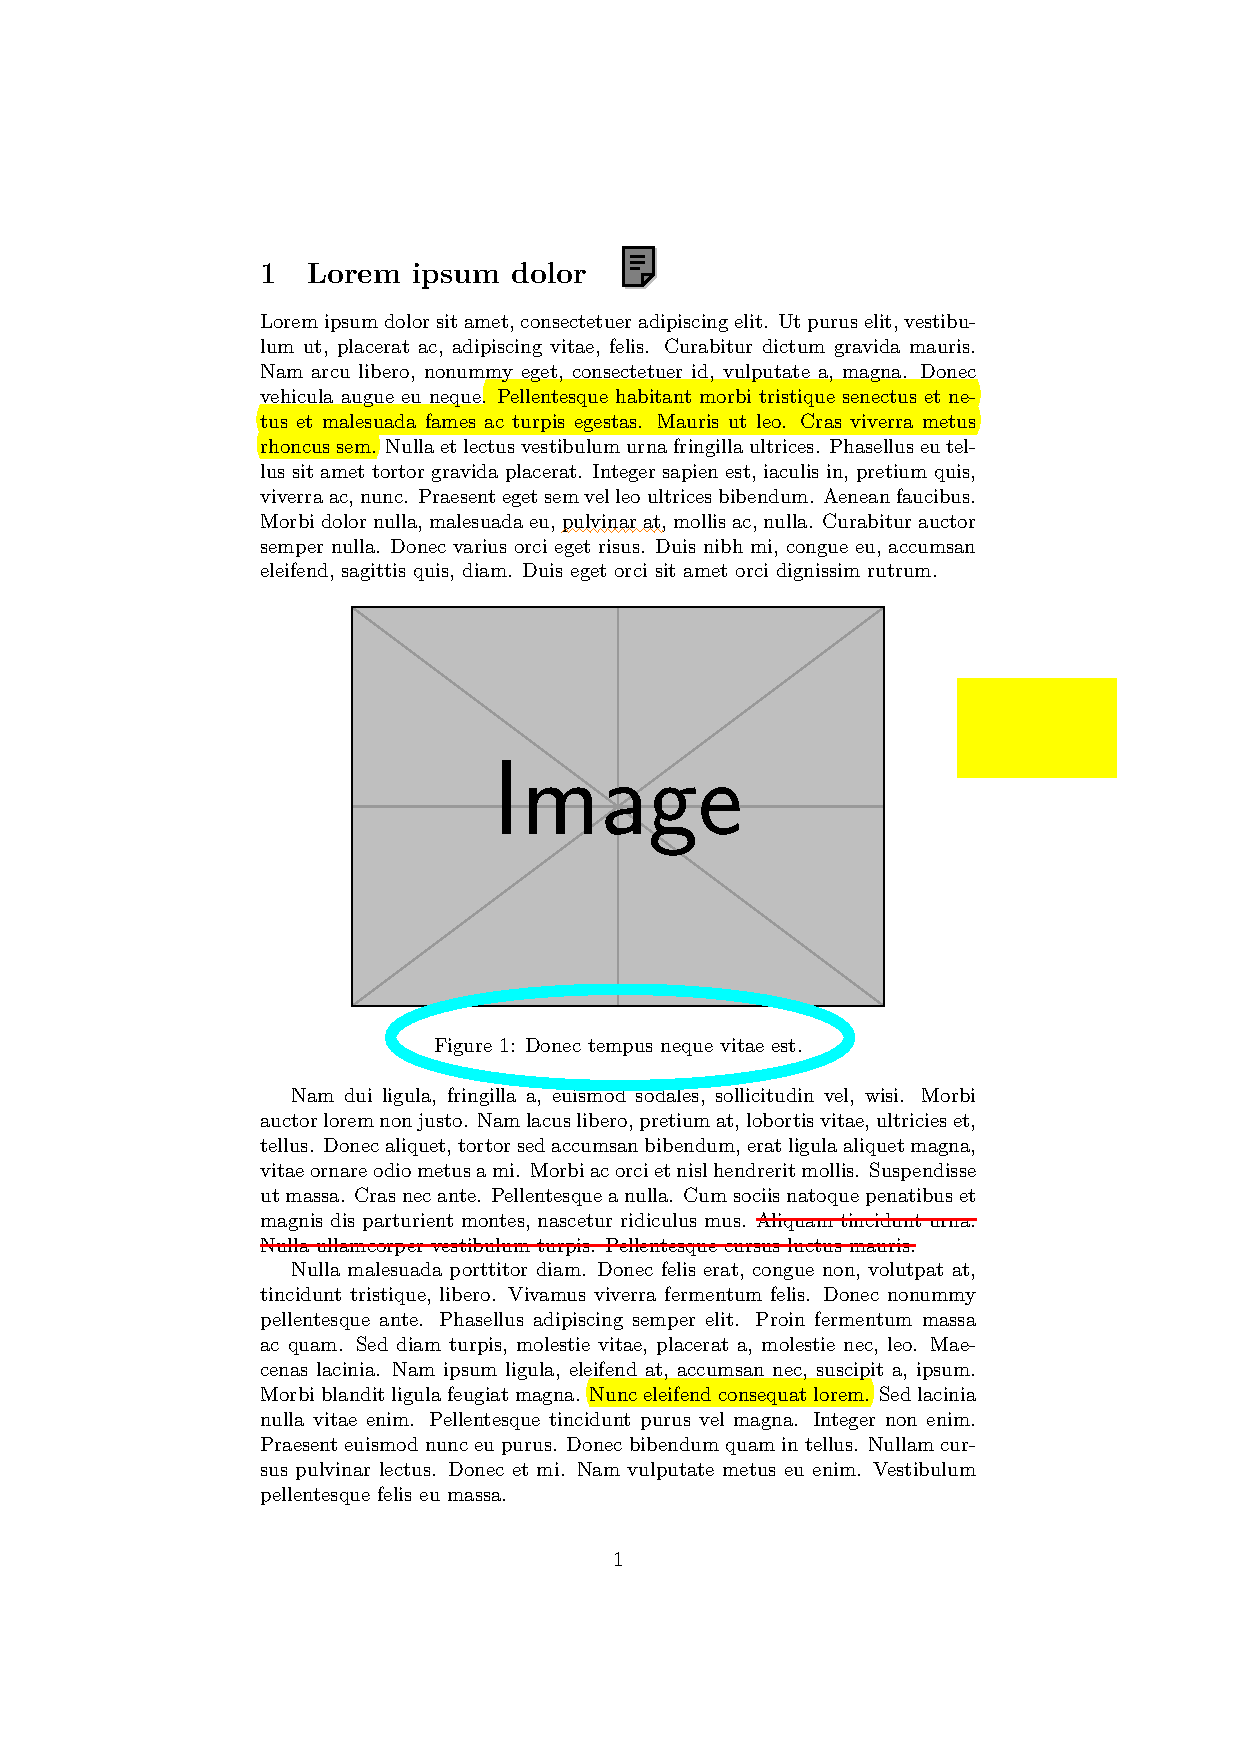
\includegraphics[
       scale=0.5,
       flareRemove!4,
       flareRemove!6
    ]{dummy-1.pdf}
  \end{lstlisting}
  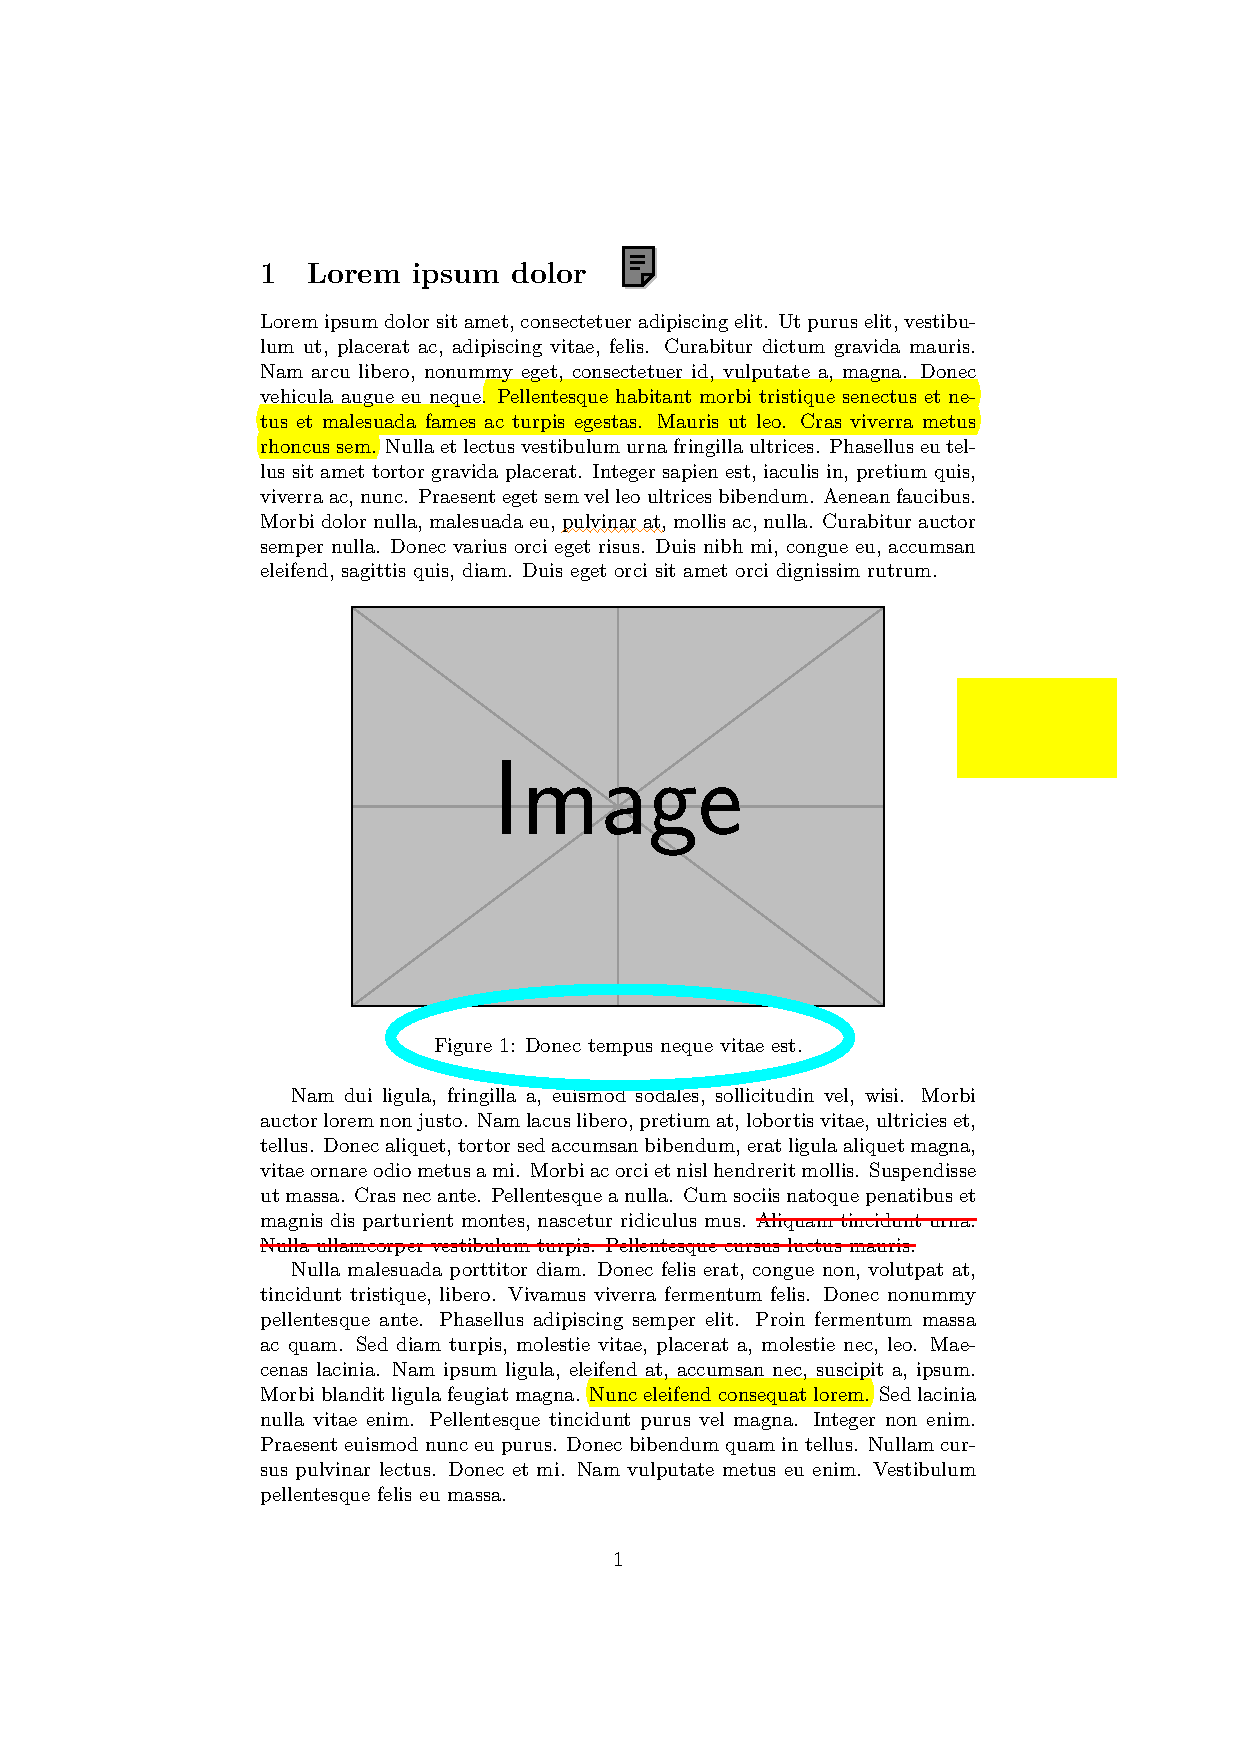
\includegraphics[
  scale=0.5,
  flareRemove!4,
  flareRemove!6
  ]{dummy-1.pdf}
\end{example}

\end{document}

%%% Local Variables:
%%% mode: latex
%%% TeX-master: t
%%% End:
